\refstepcounter{section}
\section*{Lecture 17: Einstein Field Equation}
\addcontentsline{toc}{section}{Lecture 17: Einstein Field Equation}
In Eq. \ref{eqn:EHact}, we had given a form of the Einstein-Hilbert action for gravity. Since the universe consists of matter also, the total action for the Universe is written as:
$$\Ss[\psi, g] = \Ss_{\mathrm{EH}}[g] + \Ss_{\mathrm{M}}[\psi,g]$$
where $\Ss_{\mathrm{M}}$ denotes the action for any matter field $\psi$, like electromagnetic field, fermionic and bosonic fields, etc.
To obtain the equation of motion for the metric, we have to then vary this action, that is, 
$$\delta \Ss =\frac{1}{16\pi G}\int \dd^4 x \delta \qty(\detm\ g^{\mu\nu}R_{\mu\nu}) +\delta \Ss_{\mathrm{M}}$$
To find the variation, we need to see some identitites regarding the variation of the metric. 
\begin{tcolorbox}[colframe=black, colback=lime!20!white, boxrule=1.5pt, arc=4pt]
Show the following things:
\begin{itemize} 
    \item $\delta\mathfrak{g} = \mathfrak{g}\ g^{\mu\nu}\delta g_{\mu\nu} = -\mathfrak{g} \ g_{\mu\nu}\delta g^{\mu\nu} $
    \item $\delta(\detm) = -\frac{1}{2}\detm \ g_{\mu\nu}\delta g^{\mu\nu}$
    \item $g^{\mu\nu}\delta R_{\mu\nu} = \nabla_\mu A^\mu \quad \text{where}\quad A^\mu = g^{\alpha\beta}\delta\chris{\mu}{\alpha}{\beta} - g^{\mu\nu}\chris{\rho}{\nu}{\rho} $
\end{itemize}
\end{tcolorbox}
\noindent
$\vartriangleright$ To show the first identity, let us use the Jacobi relation for a matrix $M$ that we had derived earlier:
$$\Tr ( M^{-1}\dd M) = \dd (\ln \det M)$$
Using the formula for the metric $g$, we obtain the following
$$\Tr(g^{-1}\delta g) = \frac{1}{\mathfrak{g}}\delta \mathfrak{g} \implies \delta \mathfrak{g} ={\mathfrak{g}}\tensor{{ \qty(g^{-1}\delta g)}}{^\mu _\mu} = {\mathfrak{g}} \ g^{\mu\nu}\delta g_{\nu\mu}$$
Now consider the following obvious identity, 
$$g^{-1} g = \mathds{1}$$
Taking the variation of the above (using product rule) we obtain:
$$\delta g^{-1} \ g + g^{-1} \ \delta g = 0$$
Taking the trace of the above, we obtain the other part of the identity:
\begin{align*}
    \Tr(g^{-1} \ \delta g)= -\Tr (\delta g^{-1} \ g) =  - \tensor{{ \qty(\delta g^{-1}\ g)}}{^\mu _\mu} = -\delta g^{\mu\nu}g_{\nu\mu}
\end{align*}
$\vartriangleright$ For the second identity, using the previous identity we have:
$$\delta \detm = -\frac{1}{2\detm} \delta \mathfrak{g} = -\frac{1}{2\detm} \times \qty(-\mathfrak{g}\ g_{\mu\nu}\delta g^{\mu\nu}) = -\frac{1}{2}\detm \  g_{\mu\nu}\delta g^{\mu\nu}$$
$\vartriangleright$ For the third identity, since this contains the Ricci tensor, we will start from its definition as the contracted form of the Riemann tensor:
\begin{align*}
   \delta R_{\lambda\nu} =  \delta \tensor{R}{^\rho _{\lambda\rho\nu}} &=\delta\qty(\partial_\rho\chris{\rho}{\nu}{\lambda} + \chris{\rho}{\rho}{\sigma}\chris{\sigma}{\nu}{\lambda} - \partial_\nu\chris{\rho}{\rho}{\lambda} - \chris{\rho}{\nu}{\sigma}\chris{\sigma}{\rho}{\lambda}) \\
   &=\partial_\rho \delta\chris{\rho}{\nu}{\lambda} + \delta(\chris{\rho}{\rho}{\sigma}\chris{\sigma}{\nu}{\lambda}) - \partial_\nu \delta\chris{\rho}{\rho}{\lambda} -\delta( \chris{\rho}{\nu}{\sigma}\chris{\sigma}{\rho}{\lambda})\\
   &=\mathcolor{blue}{\partial_\rho \delta\chris{\rho}{\nu}{\lambda}} + \mathcolor{red}{\delta\chris{\rho}{\rho}{\sigma}\chris{\sigma}{\nu}{\lambda}} +\mathcolor{blue}{\delta\chris{\sigma}{\nu}{\lambda} \chris{\rho}{\rho}{\sigma}}- \mathcolor{red}{\partial_\nu \delta\chris{\rho}{\rho}{\lambda}} - \mathcolor{blue}{\delta \chris{\rho}{\nu}{\sigma}\chris{\sigma}{\rho}{\lambda}} -\mathcolor{red}{\delta \chris{\sigma}{\rho}{\lambda} \delta  \chris{\rho}{\nu}{\sigma}}
\end{align*}
Now, consider the covariant derivative of the variation of the Christoffel symbol which is given as:
\begin{align*}
    \nabla_\rho (\delta \chris{\rho}{\nu}{\lambda}) &=  \mathcolor{blue}{\partial_\rho (\delta \chris{\rho}{\nu}{\lambda})} + \underbrace{\mathcolor{blue}{\chris{\rho}{\rho}{\sigma}\delta \chris{\sigma}{\nu}{\lambda}}}_{\text{for $\rho$ index}}-
   \underbrace{ \mathcolor{OliveGreen}{\chris{\sigma}{\rho}{\nu}\delta \chris{\rho}{\sigma}{\lambda}}}_{\text{for $\nu$ index}}-\underbrace{\mathcolor{blue}{\chris{\sigma}{\rho}{\lambda}\delta \chris{\rho}{\nu}{\sigma}}}_{\text{for $\lambda$ index}} \\
 \nabla_\nu (\delta \chris{\rho}{\rho}{\lambda}) &=  \mathcolor{red}{\partial_\nu (\delta \chris{\rho}{\rho}{\lambda})} + \underbrace{\mathcolor{red}{\chris{\rho}{\nu}{\sigma}\delta \chris{\sigma}{\rho}{\lambda}}}_{\text{for $\rho$ index}}-
   \underbrace{ \mathcolor{OliveGreen}{\chris{\sigma}{\nu}{\rho}\delta \chris{\rho}{\sigma}{\lambda}}}_{\text{for $\rho$ index}}-\underbrace{\mathcolor{red}{\chris{\sigma}{\nu}{\lambda}\delta \chris{\rho}{\rho}{\sigma}}}_{\text{for $\lambda$ index}}
\end{align*}
Thus, the variation of the Ricci tensor can be written as the difference of the two covariant derivatives: 
$$\delta R_{\lambda\nu} = \nabla_\rho (\delta \chris{\rho}{\nu}{\lambda}) - \nabla_\nu (\delta \chris{\rho}{\rho}{\lambda})$$
Contracting with the metric $g^{\lambda\nu}$ and noting that the metric is covariantly conserved (i.e, $\nabla_\alpha g^{\mu\nu}=0$), we have:
$$g^{\lambda\nu}\delta R_{\lambda\nu} = \nabla_\rho (g^{\lambda\nu}\delta \chris{\rho}{\nu}{\lambda}) - \nabla_\nu (g^{\lambda\nu}\delta \chris{\rho}{\rho}{\lambda}) = \nabla_\mu (g^{\lambda\nu}\delta \chris{\mu}{\nu}{\lambda}) - \nabla_\mu (g^{\lambda\mu}\delta \chris{\rho}{\rho}{\lambda})$$
where we have renamed the dummy indices in the covariant derivative. From this, we finally obtain the identity:
$$g^{\lambda\nu}\delta R_{\lambda\nu} = \nabla_\mu \qty(g^{\lambda\nu}\delta \chris{\mu}{\nu}{\lambda} - g^{\lambda\mu}\delta \chris{\rho}{\rho}{\lambda}) = \nabla_\mu A^\mu$$ \qed\\
We are finally ready to find the variation of the action to find the equation of motion. 
\begin{align*}
    \frac{1}{16\pi G}\int \dd^4 x \qty{\qty(\ -\frac{1}{2}\detm \ g_{\mu\nu}\delta g^{\mu\nu}) g^{\mu\nu}R_{\mu\nu} +\detm\ \delta g^{\mu\nu}R_{\mu\nu} +  \detm\ g^{\mu\nu}\delta R_{\mu\nu}} +\delta \Ss_{\mathrm{M}} =0
\end{align*}
The third term in the integral is equal to $\detm g^{\mu\nu}\delta R_{\mu\nu} = \detm \ \nabla_\mu A^\mu = \partial_\mu (\detm A^\mu)$ from the identity that we had proved earlier in Lec. \ref{lec:14}. This term then becomes a total derivative and vanishes at the boundary. Thus, we are left with the following,
\begin{align*}
    \int \dd^4 x\ \detm \qty[-\frac{1}{2}g_{\mu\nu}R +R_{\mu\nu}]\delta g^{\mu\nu} + 16\pi G \delta \Ss_{\mathrm{M}}=0
\end{align*}
Let us define a tensor in the following way using the functional derivative of the action for matter:
$$\ST_{\mu\nu} = -\frac{2}{\detm} \frac{\delta \Ss_{\mathrm{M}}}{\delta g^{\mu\nu}} \implies  \delta \Ss_{\mathrm{M}} = \int \dd^4x\ \frac{\delta \Ss_{\mathrm{M}}}{\delta g^{\mu\nu}}\delta g^{\mu\nu} = -\frac{1}{2}\int \dd^4 x \ \detm \ \ST_{\mu\nu}\delta g^{\mu\nu}$$
Substituting this above, we obtain:
\begin{align*}
    \int \dd^4 x\ \detm \qty[-\frac{1}{2}g_{\mu\nu}R +R_{\mu\nu} - 8\pi G \ST_{\mu\nu}]\delta g^{\mu\nu} =0
\end{align*} 
Since the metric variation is arbitrary, we have the equation of motion as:
$$\boxed{G_{\mu\nu} \equiv R_{\mu\nu} -\frac{1}{2}g_{\mu\nu}R = 8\pi G \ST_{\mu\nu}} $$
This equation is called \textit{Einstein's field equation} for material medium. The tensor, which was defined ad-hoc, is the \textit{energy-momentum tensor}. Since $G_{\mu\nu}$ is covariantly conserved, the field equation implies that so is $\ST_{\mu\nu}$, that is, $\nabla^\mu \ST_{\mu\nu} = 0$. If we also include the \textit{cosmological constant}, then we have the Einstein field equation as:
$$G_{\mu\nu} + \Lambda g_{\mu\nu} = 8\pi G \ST_{\mu\nu}$$
The above equation relates the geometry of space to the matter present, in other words, a new description of gravity. We thus hope that Newton's law could be recovered in an appropriate limit from the equation. 
\subsection{Motion of Planet around the Sun}
Consider a planet of mass $m$ orbiting around a star of mass $M>>m$ and radius $R$ at the origin. In the Newtonian case, the gravitational force and the corresponding potential  is given by $$\tvec{F} = -\frac{GMm}{r^2}\hat{\vb{r}}\qquad V_{\mathrm{N}} = \frac{-GMm}{r}$$
\begin{figure}[H]
    \centering 


% Gradient Info
  
\tikzset {_gpnpu7fmy/.code = {\pgfsetadditionalshadetransform{ \pgftransformshift{\pgfpoint{0 bp } { 0 bp }  }  \pgftransformrotate{0 }  \pgftransformscale{2 }  }}}
\pgfdeclarehorizontalshading{_i3pg9w1ze}{150bp}{rgb(0bp)=(1,0.99,0.92);
rgb(37.5bp)=(1,0.99,0.92);
rgb(62.5bp)=(0.95,0.85,0.21);
rgb(100bp)=(0.95,0.85,0.21)}

% Gradient Info
  
\tikzset {_t3lf7s59t/.code = {\pgfsetadditionalshadetransform{ \pgftransformshift{\pgfpoint{0 bp } { 0 bp }  }  \pgftransformrotate{0 }  \pgftransformscale{2 }  }}}
\pgfdeclarehorizontalshading{_9rnygfxw7}{150bp}{rgb(0bp)=(0.82,0.89,0.97);
rgb(37.5bp)=(0.82,0.89,0.97);
rgb(43.5bp)=(0.45,0.69,0.91);
rgb(50bp)=(0.04,0.47,0.84);
rgb(57.25bp)=(0.33,0.62,0.88);
rgb(62.5bp)=(0.53,0.74,0.92);
rgb(100bp)=(0.53,0.74,0.92)}
\tikzset{every picture/.style={line width=0.75pt}} %set default line width to 0.75pt        

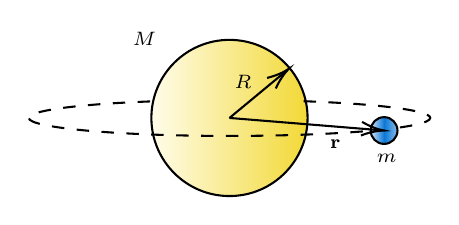
\begin{tikzpicture}[x=0.75pt,y=0.75pt,yscale=-1,xscale=1]
%uncomment if require: \path (0,150); %set diagram left start at 0, and has height of 150

%Shape: Circle [id:dp9887170448190994] 
\path  [shading=_i3pg9w1ze,_gpnpu7fmy] (190.43,70.09) .. controls (190.43,49.31) and (207.28,32.47) .. (228.06,32.47) .. controls (248.84,32.47) and (265.68,49.31) .. (265.68,70.09) .. controls (265.68,90.87) and (248.84,107.72) .. (228.06,107.72) .. controls (207.28,107.72) and (190.43,90.87) .. (190.43,70.09) -- cycle ; % for fading 
 \draw   (190.43,70.09) .. controls (190.43,49.31) and (207.28,32.47) .. (228.06,32.47) .. controls (248.84,32.47) and (265.68,49.31) .. (265.68,70.09) .. controls (265.68,90.87) and (248.84,107.72) .. (228.06,107.72) .. controls (207.28,107.72) and (190.43,90.87) .. (190.43,70.09) -- cycle ; % for border 

%Shape: Arc [id:dp5853203999346669] 
\draw  [draw opacity=0][dash pattern={on 4.5pt off 4.5pt}] (263.75,62.03) .. controls (299.51,63.31) and (324.79,66.43) .. (324.79,70.09) .. controls (324.79,74.88) and (281.48,78.76) .. (228.06,78.76) .. controls (174.63,78.76) and (131.33,74.88) .. (131.33,70.09) .. controls (131.33,66.49) and (155.8,63.41) .. (190.64,62.1) -- (228.06,70.09) -- cycle ; \draw  [dash pattern={on 4.5pt off 4.5pt}] (263.75,62.03) .. controls (299.51,63.31) and (324.79,66.43) .. (324.79,70.09) .. controls (324.79,74.88) and (281.48,78.76) .. (228.06,78.76) .. controls (174.63,78.76) and (131.33,74.88) .. (131.33,70.09) .. controls (131.33,66.49) and (155.8,63.41) .. (190.64,62.1) ;  
%Shape: Circle [id:dp1865453991829401] 
\path  [shading=_9rnygfxw7,_t3lf7s59t] (296.1,76.15) .. controls (296.1,72.59) and (298.99,69.7) .. (302.55,69.7) .. controls (306.11,69.7) and (309,72.59) .. (309,76.15) .. controls (309,79.71) and (306.11,82.6) .. (302.55,82.6) .. controls (298.99,82.6) and (296.1,79.71) .. (296.1,76.15) -- cycle ; % for fading 
 \draw   (296.1,76.15) .. controls (296.1,72.59) and (298.99,69.7) .. (302.55,69.7) .. controls (306.11,69.7) and (309,72.59) .. (309,76.15) .. controls (309,79.71) and (306.11,82.6) .. (302.55,82.6) .. controls (298.99,82.6) and (296.1,79.71) .. (296.1,76.15) -- cycle ; % for border 

%Straight Lines [id:da779039052259979] 
\draw    (228.06,70.09) -- (300.56,75.99) ;
\draw [shift={(302.55,76.15)}, rotate = 184.65] [color={rgb, 255:red, 0; green, 0; blue, 0 }  ][line width=0.75]    (10.93,-3.29) .. controls (6.95,-1.4) and (3.31,-0.3) .. (0,0) .. controls (3.31,0.3) and (6.95,1.4) .. (10.93,3.29)   ;
%Straight Lines [id:da13332950074843586] 
\draw    (228.06,70.09) -- (255.14,47.66) ;
\draw [shift={(256.68,46.38)}, rotate = 140.37] [color={rgb, 255:red, 0; green, 0; blue, 0 }  ][line width=0.75]    (10.93,-3.29) .. controls (6.95,-1.4) and (3.31,-0.3) .. (0,0) .. controls (3.31,0.3) and (6.95,1.4) .. (10.93,3.29)   ;

% Text Node
\draw (275,79.1) node [anchor=north west][inner sep=0.75pt]  [font=\scriptsize]  {$\mathbf{r}$};
% Text Node
\draw (229,48.1) node [anchor=north west][inner sep=0.75pt]  [font=\scriptsize]  {$R$};
% Text Node
\draw (180,27.1) node [anchor=north west][inner sep=0.75pt]  [font=\scriptsize]  {$M$};
% Text Node
\draw (297.55,86) node [anchor=north west][inner sep=0.75pt]  [font=\scriptsize]  {$m$};


\end{tikzpicture}

\end{figure}
\textbf{Properties of the Newtonian gravity:}\\
\begin{itemize}
    \item Since the acceleration has second order derivative in time, the equation has \underline{time-reversal symmetry}.
    \item The planets move through a \underline{matter free-region} in space (for $r>R$) which means that $\ST_{\mu\nu}(\vb{x})=0$ in the exterior part of the star, that is, along the orbit where the planets move. 
    \item Since the potential do not depend on $\theta$ and $\phi$ angles, the potential is \underline{spherically-symmetric}.
    \item Since the potential is \underline{time-independent}, there is no dynamics associated with the field and hence the field is \textit{static}. 
\end{itemize}
Considering the above properties, we must look for a spherically symmetric, time-independent and stationary vacuum solution to the field equation which also enjoys time reversal symmetry. It is kinda obvious that the appropriate coordinates to work with are $(t,r,\theta,\phi)$ which are called the \textit{Schwarzschild coordinates}. In terms of these coordinates, the most general metric is:
\begin{align*}
    ds^2 = g_{\mu\nu} \dd x^\mu \dd x^\nu &= \qty{g_{tt}\ \dd t^2  +2(g_{tr}\ \dd t\ \dd r +g_{t\theta}\ \dd t\ \dd \theta+g_{t\phi}\ \dd t\ \dd \phi ) } \\
    &+\qquad \qty{g_{rr}\ \dd r^2  +2(g_{r\theta}\ \dd r\ \dd \theta+g_{r\phi}\ \dd r\ \dd \phi) } +  \qty{g_{\theta\theta}\ \dd \theta^2 + 2g_{\theta\phi}\ \dd \theta \dd \phi} + g_{\phi\phi}\ \dd \phi^2
\end{align*}
Invoking spherical symmetric, we expect that at a particular $t_o$ and fixed radius $r_o$, the metric should reduce to the metric on $\mathbb{S}^2$ which we had derived earlier. Thus, 
$$ds^2\Big|_{r_o,t_o} = r_o^2\ \dd \theta^2 + r_o^2\sin^2\theta\ \dd \phi^2$$
From which we can say that the metric elements will be: $$ g_{\theta\phi} = 0\quad g_{\phi\phi}= r^2\sin^2\theta\quad  g_{\theta\theta} = r^2 $$
The metric should also be independent of the orientation in $\theta$ and $\phi$ since we expect spherically symmetric solutions. Hence, the metric must remain invariant under $\theta\to -\theta$ and $\phi \to -\phi$, from which we obtain:
$$g_{t\theta} = 0 \ g_{r\theta}=0\ g_{t\phi} = 0 \ g_{r\phi}=0 $$
These symmetry considerations significantly reduced the metric. We presently have:
$$ds^2 = g_{tt}\ \dd t^2 + 2g_{tr}\ \dd t \ \dd r +g_{rr}\ \dd r^2+ r^2\qty(\dd \theta^2 + \sin^2\theta \ \dd \phi^2)$$
From the time-independent consideration, we can say that none of the metric tensor components must depend on time. They should only depend on $r$ (since spherical symmetry is also there). And under time-reversal, the metric should be invariant under $t\to -t$ from which we have $g_{tr=0}$. Let us denote $g_{tt} = f(r)$ and $g_{rr}=h(r)$. The final expression of the metric, in terms of the two unknowns $f(r)$ and $h(r)$ becomes:
$$\boxed{ds^2 = f(r)\ \dd t^2 +h(r)\ \dd r^2+ r^2\qty(\dd \theta^2 + \sin^2\theta \ \dd \phi^2)}$$
The above metric is the only unique spherically symmetric solution to the vacuum Einstein field equation which is stated in \textit{Birkhoff's Theorem}.